\subsubsection*{Analysis}
\begin{tabular}{@{}l l}
\textbf{Scope}:&The AuctionHouse\textsuperscript{TM} automated administration system\\
\textbf{Level}:&User goal\\
\textbf{Primary Actor}:&Purchasing Agent, Auctioneer, Secretary\\
\textbf{Stakeholders and Interests}:&\begin{tabular}[t]{@{}l}Purchasing Agent, Auctioneer, Secretary: wants to update item parameters quickly and easly.\end{tabular}\\
\textbf{Preconditions}:&Actor is identified and authenticated.\\
\textbf{Postconditions}:&\begin{tabular}[t]{@{}l}The item has been updated on the system, or a failure was returned.\\The updates to the item are (or will become) visible for potential buyers\\and the otherwise authorized.\end{tabular}\\
\textbf{Special requirements}:&\begin{tabular}[t]{@{}l}The current information of an item and a list of future auction dates needs to available\\in the system.\end{tabular}\\
\textbf{Frequency of occurence}:&Frequent\\
\end{tabular}\\\\
\textsl{Main Success Scenario}
\begin{enumerate}[noitemsep]
	\item The user starts the transaction.
	\item The system provides the user with the current information of the item that they are authorised to edit.
	\item The user provides the updated information. The information that can be updated is
	\begin{itemize}[noitemsep]
		\item The amount of the item available
		\item The type of item
		\item A description
		\item If the item possesses any antiquarian value
		\item A minimum price decided by the owner
		\item The date when brought in
		\item Name and address of the owner plus identification
		\item Planned auction date
		\item Distinguishing features
	\end{itemize}
	\item The system updates the item with the given information.
	\item The system returns to the user whether it was successful.
\end{enumerate}
\textsl{Extensions}
\begin{itemize}[noitemsep]
	\item If unsucessful, the system database remains unchanged; no item or other information was added or changed.
\end{itemize}
\textsl{System Sequence Diagram}
\begin{figure}[H]
	\centering
	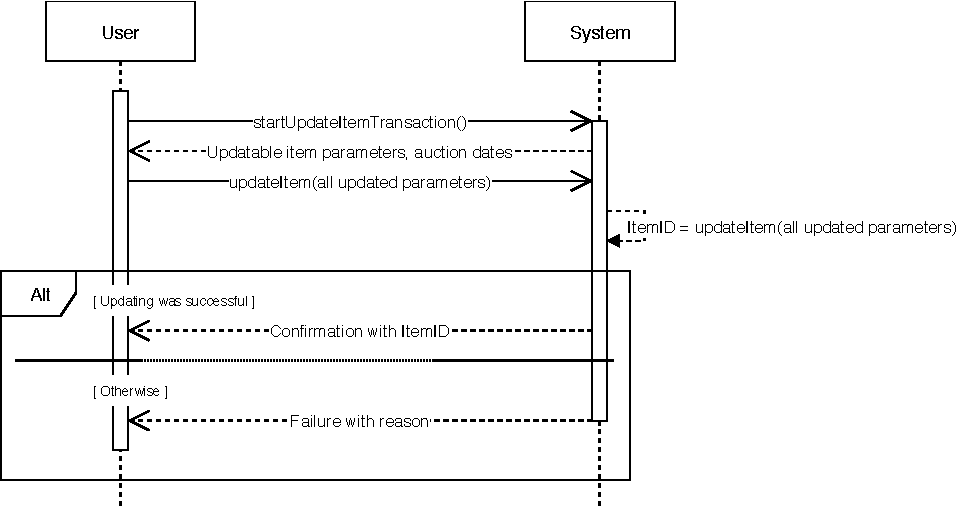
\includegraphics[scale=1]{SD-bb-update.pdf}
	\caption*{Interactions displayed in a System Sequence Diagram in blackbox format}
\end{figure}